\subsubsection{Taxi Driver Availability Notification}
			To accompany this diagram, read the Scenario \hyperref[sec:TaxiDriverAvailabilityScenario]{S.13}.

				\begin{table}[htpb]
					\centering
					\label{tab:TaxiDriverAvailabilityTable}
					\begin{tabularx}{\textwidth}{lp{9cm}}
						\hline
						\hline
							\textbf{Subject}
						& 
							\textbf{Description}\\
						\hline
							Actors	       &  Taxi Driver, myTaxiService Mobile Application, myTaxiService Server\\
						\hline
							Preconditions  &  Taxi Driver must be on the homepage and must be already logged in. Taxi Driver must not be already available on the system.\\
						\hline
							Execution      &  1.~Taxi Driver taps on the "Available" ON/OFF button.\\
										   &  2.~myTaxiService Mobile Application calls the relative server function.\\
										   &  3.~myTaxiService Server sets the Taxi Driver to available and adds him to the zone queue.\\
										   &  4.~myTaxiService Server notifies the Application of the result.\\
										   &  5.~myTaxiService Mobile Application shows to the Taxi Driver that he's now available on the system.\\
						\hline
							Postconditions &  The Taxi Driver is now available for the system.\\
						\hline
							Exceptions     &  2.~The Taxi Driver disconnects before the server response.\\
									
						\hline
						\hline
					\end{tabularx}
				\end{table}
				
				\begin{figure}[H]
					\centering
					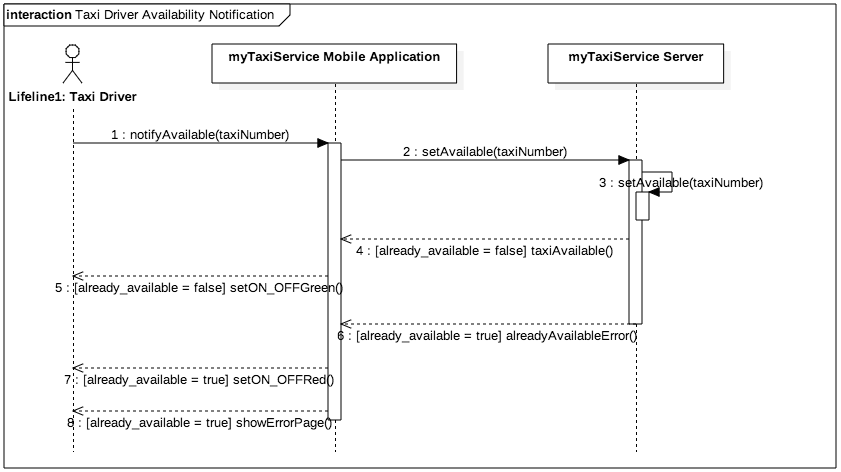
\includegraphics[width=\textwidth, scale=0.5]{IMG/InteractionDiagrams/TaxiDriverAvailability.png}
					\caption{Reservation Deletion Interaction Diagram}\label{sec:FigureTaxiDriverAvailability}
				\end{figure}